\documentclass{article}
\usepackage{wasysym}
\usepackage{graphics}
\usepackage{psfig}
\usepackage{epsfig}
\newcommand{\bc}{\begin{center}}
\newcommand{\ec}{\end{center}}
\newcommand{\be}{\begin{equation}}
\newcommand{\ee}{\end{equation}}
\newcommand{\bea}[1]{\begin{eqnarray}\label{#1}}
\newcommand{\eea}{\end{eqnarray}}
\newcommand{\bua}{\begin{eqnarray*}}
\newcommand{\eua}{\end{eqnarray*}}
\newcommand{\dd}[2]{{{d^2#1}\over{d#2^2}}}
\newcommand{\aver}[1]{\langle{#1}\rangle}
\def\cl#1{{\cal #1}}               % for caligrafic letters
\def\abs{\!\mid\!}
\def\labs{\mid\!}
\def\rabs{\!\mid}
\def\rd{\mbox{d}}
\def\rD{\mbox{D}}
\begin{document}
\section*{Lecture notes 3: Detectors}

\subsection*{Detector parameters}

The overall performance of a detector (CCD or other) is described in terms of
different technical parameters. A short-list of such parameters
include:

\begin{itemize}
  \item The {\em quantum efficiency} (QE) is the ratio of the actual
  number of photons detected to the number of incident photons. This
  quantity varies with wavelength. In the range 300-900~nm typical
  values fall in the range 0.2--0.75 with maximum efficiency around 
  500~nm.  
  \item The {\em spectral response} is the change in the output
  signal as a function of the wavelength of the input signal.
  \item The {\em charge transfer efficiency} (CTE) specifies the 
  efficiency at which accumulated charge may be transfered from one 
  pixel to the next. For a 1~\% accuracy in the read-out process 
  for a 10000 element detector a 99.9999~\% transfer efficiency is
  required. Actual numbers as high as 99.99999~\% have been quoted.
  \item The {\em dark current} represent the output from the
  non-illuminated detector. It is usually measured as a
  root-mean-square current.  
  \item The {\em dynamic range} is the ratio of the saturation output
  to the dark current.  
  \item The {\em  noise equivalent power} (NEP) is the input radiative 
  flux that gives
  a signal-to-noise ratio of unity. It may be given for monochromatic
  or black body radiation. It is usually measured in watts.  
  \item The  {\em detectivity} (D) is the inverse NEP value, that is, the
  signal-to-noise ratio for unity intensity input radiation.  
  \item  The {\em normalized detectivity} (D$^*$) is the detectivity
  normalized by multiplying with the square root of the product of the
  detector area and the electrical bandwidth of the measuring
  circuitry 
  \begin{equation} 
    D^* = \frac{(A \Delta f)^{1/2}}{NEP}.
    \label{CCD.Dstar}
  \end{equation}
  The usual unit is cm Hz$^{1/2}$ W$^{-1}$.
\end{itemize}

The technical specifications for the CCD are improving year by
year. Instead of dwelling further on such specifications or the
practical challenges met with in the fabrication process of such
devices, we will therefore turn to a discussion of the physical
principles behind the working detector. This will require knowledge of
basic properties of solid state conductors, insulators, and
semi-conductors, the photo-electric effect, and the
metal-oxide-semiconductor (MOS) capacitor.

\subsection*{Semiconductors}

Many types of detectors base their properties on those of {\it
  semiconductors}. Thus, let us discuss these properties as a
prerequisite to achieving an understanding of the detectors that
employ them. 

For a single many-electron atom the Pauli principle requires the
electrons to occupy different electron states. This principle also
applies to the total number of electrons in a solid block of
material. Instead of the discrete energy levels of the single atom,
the solid block displays a series of continuous energy bands available
to the electrons. Energy bands for which every allowed electron state
is occupied at zero temperature are called valence bands, energy bands
that are only partially filled are called conduction bands. 

From statistical mechanics the probability distribution function for
finding a given energy level $U$ occupied by an electron (of spin 1/2)
is given by the Fermi-Dirac distribution function
\begin{equation}
  f_{FP}(U) \sim \frac{1}{1+\exp((U-U_F)/\cl T)},
  \label{CCD.fFD}
\end{equation}
where $\cl T$ is the temperature (in energy units, $\cl T = \kappa T$
where $\kappa$ is the Boltzmann constant and $T$ temperature in
degrees Kelvin) and $U_F$ is the Fermi energy. The Fermi-Dirac
distribution function (\ref{CCD.fFD}) is displayed in figure
\ref{CCD.figfFD}. At $\cl T = 0$ all energy levels up to $U_F$ are
occupied. At finite temperatures a definite variation of $f_{FD}$ with
$U$ is found only for $\labs U - U_F \rabs$-values up to order $\cl
T$. We note that $U_F$ represents the average energy acquired by an
extra electron introduced to the material block under conditions of
constant temperature. With the zero of the energy scale referred to the
usual infinity of vacuum electrostatics, the Fermi energy is also
referred to as the electro-chemical potential of the electron.

\begin{figure}[h]
  \centering  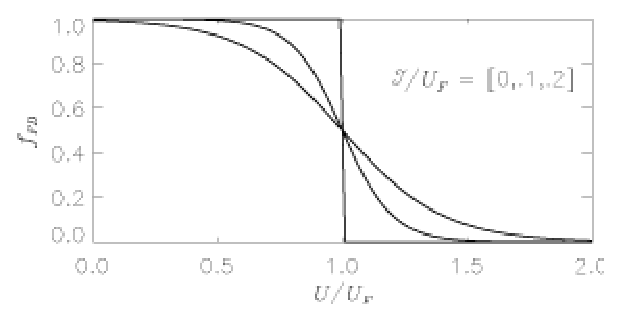
\includegraphics{CCD_fFD.eps}
  \caption{The Fermi-Dirac distribution function}
  \label{CCD.figfFD}
\end{figure}

If an electric field is imposed on the material, the electrons will
tend to move. In this process the energy of the electron must
increase, the extra energy later to be expended in collisions with
other electrons or sound generation, and leading to the Ohmic heating
of the material. For an electron to increase its energy, however, a
suitable empty local energy level must be available. In the absence of
such energy levels the electron is not allowed to move. In metals with
a partly filled conduction band there is ample supply of such empty
energy levels, the conduction band electrons are free to move. The
metals are therefore good electrical conductors, with the electrical
conductance generally decreasing with temperature. In figure
\ref{CCD.figsolstate} valence band energy levels are drawn blue,
conduction band levels red. Filled levels are illustrated with
solid lines, empty levels by dashed lines. 


Now consider a material made from group IV atoms like carbon (C),
silicon (Si) or germanium (Ge).  These atoms each make covalent
bindings with their four nearest neighbors. This results in filled
valence bands and an empty conduction band.  For diamond (C) the
energy gap between the top of the valence band $U_V$ and the bottom of
the conduction band $U_C$ is of the order of 6 to 7 eV, much larger
than the typical thermal energy of the topmost electrons. Thus, the
conduction band remains empty and there are no available local energy
levels for electrons in the filled valence band to move to under
influence of the electric field. The electrons are thus not allowed to
move and the material will be an insulator.

\begin{figure}[h]
  \centering  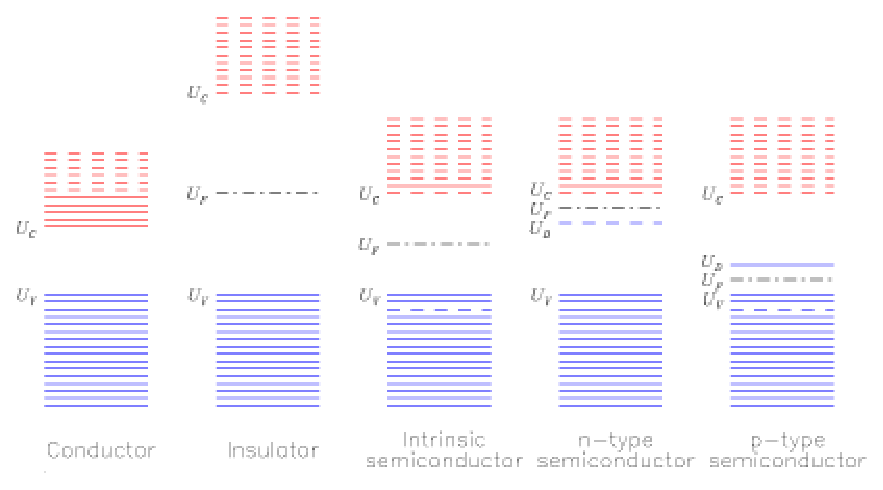
\psfig{file=CCD_solstate.eps,width=0.95\textwidth}
  \caption{Solid state energy levels}
  \label{CCD.figsolstate}
\end{figure}


For crystalline silicon the corresponding energy gaps is 1.10 eV. In
this case some of the electrons may be thermally excited to the
conduction band even at room temperature. This leaves empty energy
levels (holes) in the valence band. This means that these materials
are semiconductors with an electrical conductance strongly dependent
on (and increasing with) the temperature of the material. Charge is
transported through the material not only by the thermally excited
electrons of the conduction band. An important observation is that
even an empty hole in an otherwise filled valence band will act as a
free positively charged, charge carrier. Neighboring electrons of the
valence band may under the influence of the imposed electric field
move into the empty electron state, resulting in the motion of the
hole in the opposite direction.

The number of electrons that are excited to the conduction band is
determined by the temperature through the Fermi-Dirac
distribution. The Fermi energy will vary in accordance with the number
of thermally excited electrons, typically taking values about halfway
between $U_V$ and $U_C$. This also means that if extra electrons are
added to the semiconductor, about half of these are added to the
conduction band, the other half occupying energy levels near the top
of the valence band that are made empty. A semiconductor that has an
equal number of holes and electrons that can move under the influence
of an electric field is called an intrinsic semiconductor. This type
of semiconductors stands in contrast to semiconductors contaminated
with foreign atoms.

In a silicon crystal contaminated with group V atoms (for instance
phosphor P), each foreign atom will replace one Si atom in the crystal
lattice and remain fixed in this location. The foreign atom
contributes one extra electron relative to the Si atom it replaces and
will therefore be called a donor atom. The extra electron will occupy
what are called donor impurity levels. In figure \ref{CCD.figsolstate}
these levels are denoted $U_D$. They are found just below the
conduction band, approximately 0.05 eV from the edge of the conduction
band. We recall that this is only twice the value of $\cl T$ at room
temperature. The electrons in the donor impurity levels are thus
easily thermally excited into the conduction band, leaving behind an
ionized donor atom in the lattice. Such materials conduct almost
entirely by negative charge carriers (electrons) and are called n-type
semiconductors. Under conditions of complete ionization the number
density of free charge carriers (electrons) will be equal to the
number density $N_D$ of impurity atoms.

If the silicon crystal instead is contaminated by group III atoms (for
instance boron B) each foreign atom will lack one electron for a
complete chemical binding. Such atoms will leave vacant levels (holes)
in the valence band. These atoms are therefore called acceptors.  The
vacant levels, called acceptor impurity levels and denoted $U_A$ in
figure \ref{CCD.figsolstate}, are located just above the top of the
valence band, approximately 0.05 eV from the edge of the valence band.
Neighboring valence band electrons are easily thermally excited into
the vacant levels where they will be trapped and not allowed to
move. They do, however, leave behind holes in the valence band which
may act as positive charge carriers. Such materials are therefore
called p-type semiconductors. Again the number density of free charge
carriers (holes) will be equal to the number density $N_A$ of impurity
atoms for a state of complete ionization.

We note that at low enough temperatures ($T < 70$ K) the ionization
degrees for both types of doped semiconductors become negligible and
therefore that the materials stop to act as semiconductors. This
phenomenon is referred to as ``freeze-out''. At this point the CCD
will cease to function.

\subsection*{The photoelectric effect}

The photo-electric effect traditionally refers to a process in which
the energy $h\nu$ of a photon is absorbed by one electron in the
surface layer of a metal, and where the energized electron
subsequently escapes the metal with a maximum kinetic energy
\begin{equation}
  U_{kin} = h\nu - W.
\end{equation}
Here $W$ represents the work function of the metal, that is, the
energy needed to lift an electron from the top of the conduction band
to just outside the metal surface. The photo-electric effect is
important historically in that it clearly demonstrated the quantum
nature of light.

In the present context we are interested in the photo-electric effect
in doped semiconductors. The semiconductor will be initialized in a
completely depleted state, that is, every free charge carrier will be
driven away from the illuminated part of the material. We are
interested in the process where the photon energy $h\nu$ is absorbed
by a bounded, valence band electron, and where the electron is
lifted to the conduction band and therefore becoming a free charge
carrier in the semiconductor itself. The CCD detector relies on our 
ability to collect and subsequently count the number of such electrons
being produced.

The quantum efficiency for a CCD detector can be represented in the form
\begin{equation}
  QE = CCE(1-R_{ref}) \exp(-x_{poly}/L_A) (1-\exp(-x_{epi}/L_A))
  \label{CCD.QE}
\end{equation}
Here $CCE$ is the charge collection efficiency, that is, the ability
of the detector to collect all the photoelectrons generated. This is
often a factor of value close to unity. $R_{ref}$ is the reflection
coefficient for silicon at the wavelength of interest, and $L_A$ the
corresponding photon absorption length in the epitaxial layer of
effective thickness $x_{epi}$. The third factor in expression
(\ref{CCD.QE}) will be present for front side illuminated CCDs with
effective poly-crystalline gate thickness $x_{poly}$. 

\begin{figure}[h!]
\hfil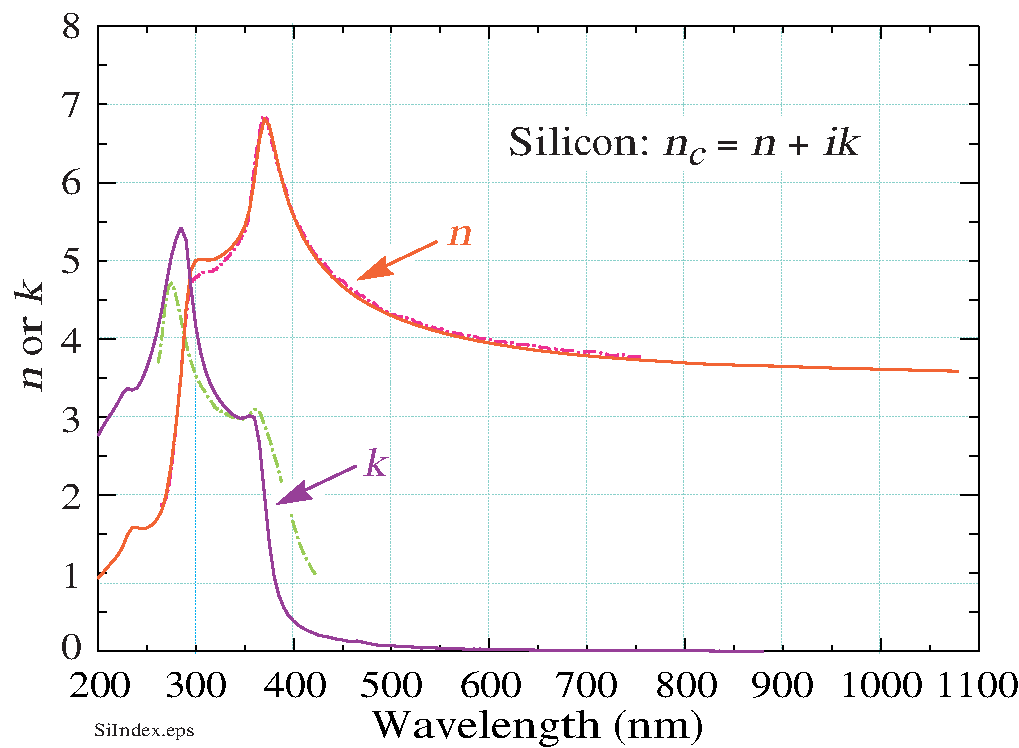
\psfig{file=SiIndex.eps,width=0.7\textwidth}\hfil
\caption{Reflection coeffecients (both real and imaginary) for Si as a function
of wavelength.}
\label{fig:si-refl}
\end{figure}

In figure~\ref{fig:si-refl} the reflection 
coefficient of silicon is plotted as a function of wavelength for the range 
200-1100~nm. In figure~\ref{fig:si-abs} the
corresponding absorption length is given for the same wavelength band.
We notice the reduced quantum efficiency in the UV to soft X-ray
range. Increased efficiency for wavelengths down to about 50~nm will
result by applying phosphor coatings to the illuminated side of the
CCD. The phosphor absorbs incoming photons of one wavelength and then
re-emits isotropically at a longer wavelength. A loss factor of 50~\%
results from the isotropic re-radiation property. A popular phosphor
is lumigen, effective for wavelengths less than 480~nm and
re-emitting at about 530~nm. 

\begin{figure}[h!]
\hfil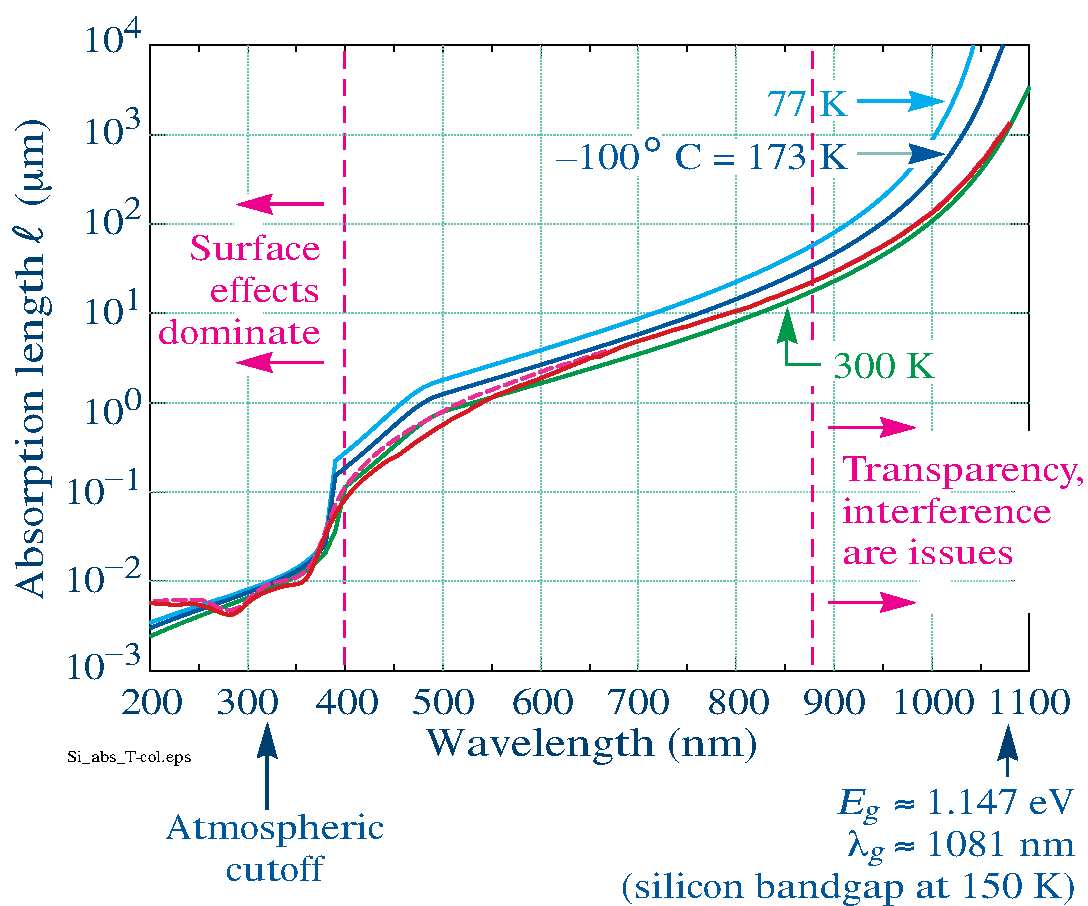
\psfig{file=Si_abs_T-col.eps,width=0.7\textwidth}\hfil
\caption{Absorption length of Si as a function of wavelength and temperature.}
\label{fig:si-abs}
\end{figure}

To be able to lift a valence-band electron to the conduction band the
photon energy $h\nu$ must exceed the band gap energy, $U_C-U_V \approx
1.1$ eV for silicon. This corresponds to wavelengths $\lambda < 1090$~nm. 
For photons with less energy silicon will appear transparent. Note in 
connection with this that the electrodes at or near the surface of a
detector such as a CCD can reflect some of the incident light thus reducing
the detectors efficiency. One solution to this is to replace 
metallic electrodes with transparent polysilicon electrodes. Alternately,
the detector may be illuminated from the back so that it does not have to
pass through the electrodes at all. This, though, requires that the silicon
forming the detector be very thin so that the electrons produced by 
incident radiation are collected efficiently. This process is difficult
and many devices may be damaged during operation. Successfully thinned
CCDs are therefore expensive as well as being fragile. At longer 
wavelengths the thinned CCD can become semi-transparent, this reduces the
efficiency of the CCD and may in addition cause interference fringes 
to be produced, which must be removed in the data reduction process. Both
of these effects are visible in figure~\ref{fig:crisp8542raw-momfbd}, which
features a solar image taken in the infrared 854.2~nm Ca~{\sc ii} line.

\begin{figure}[p]
\centering{
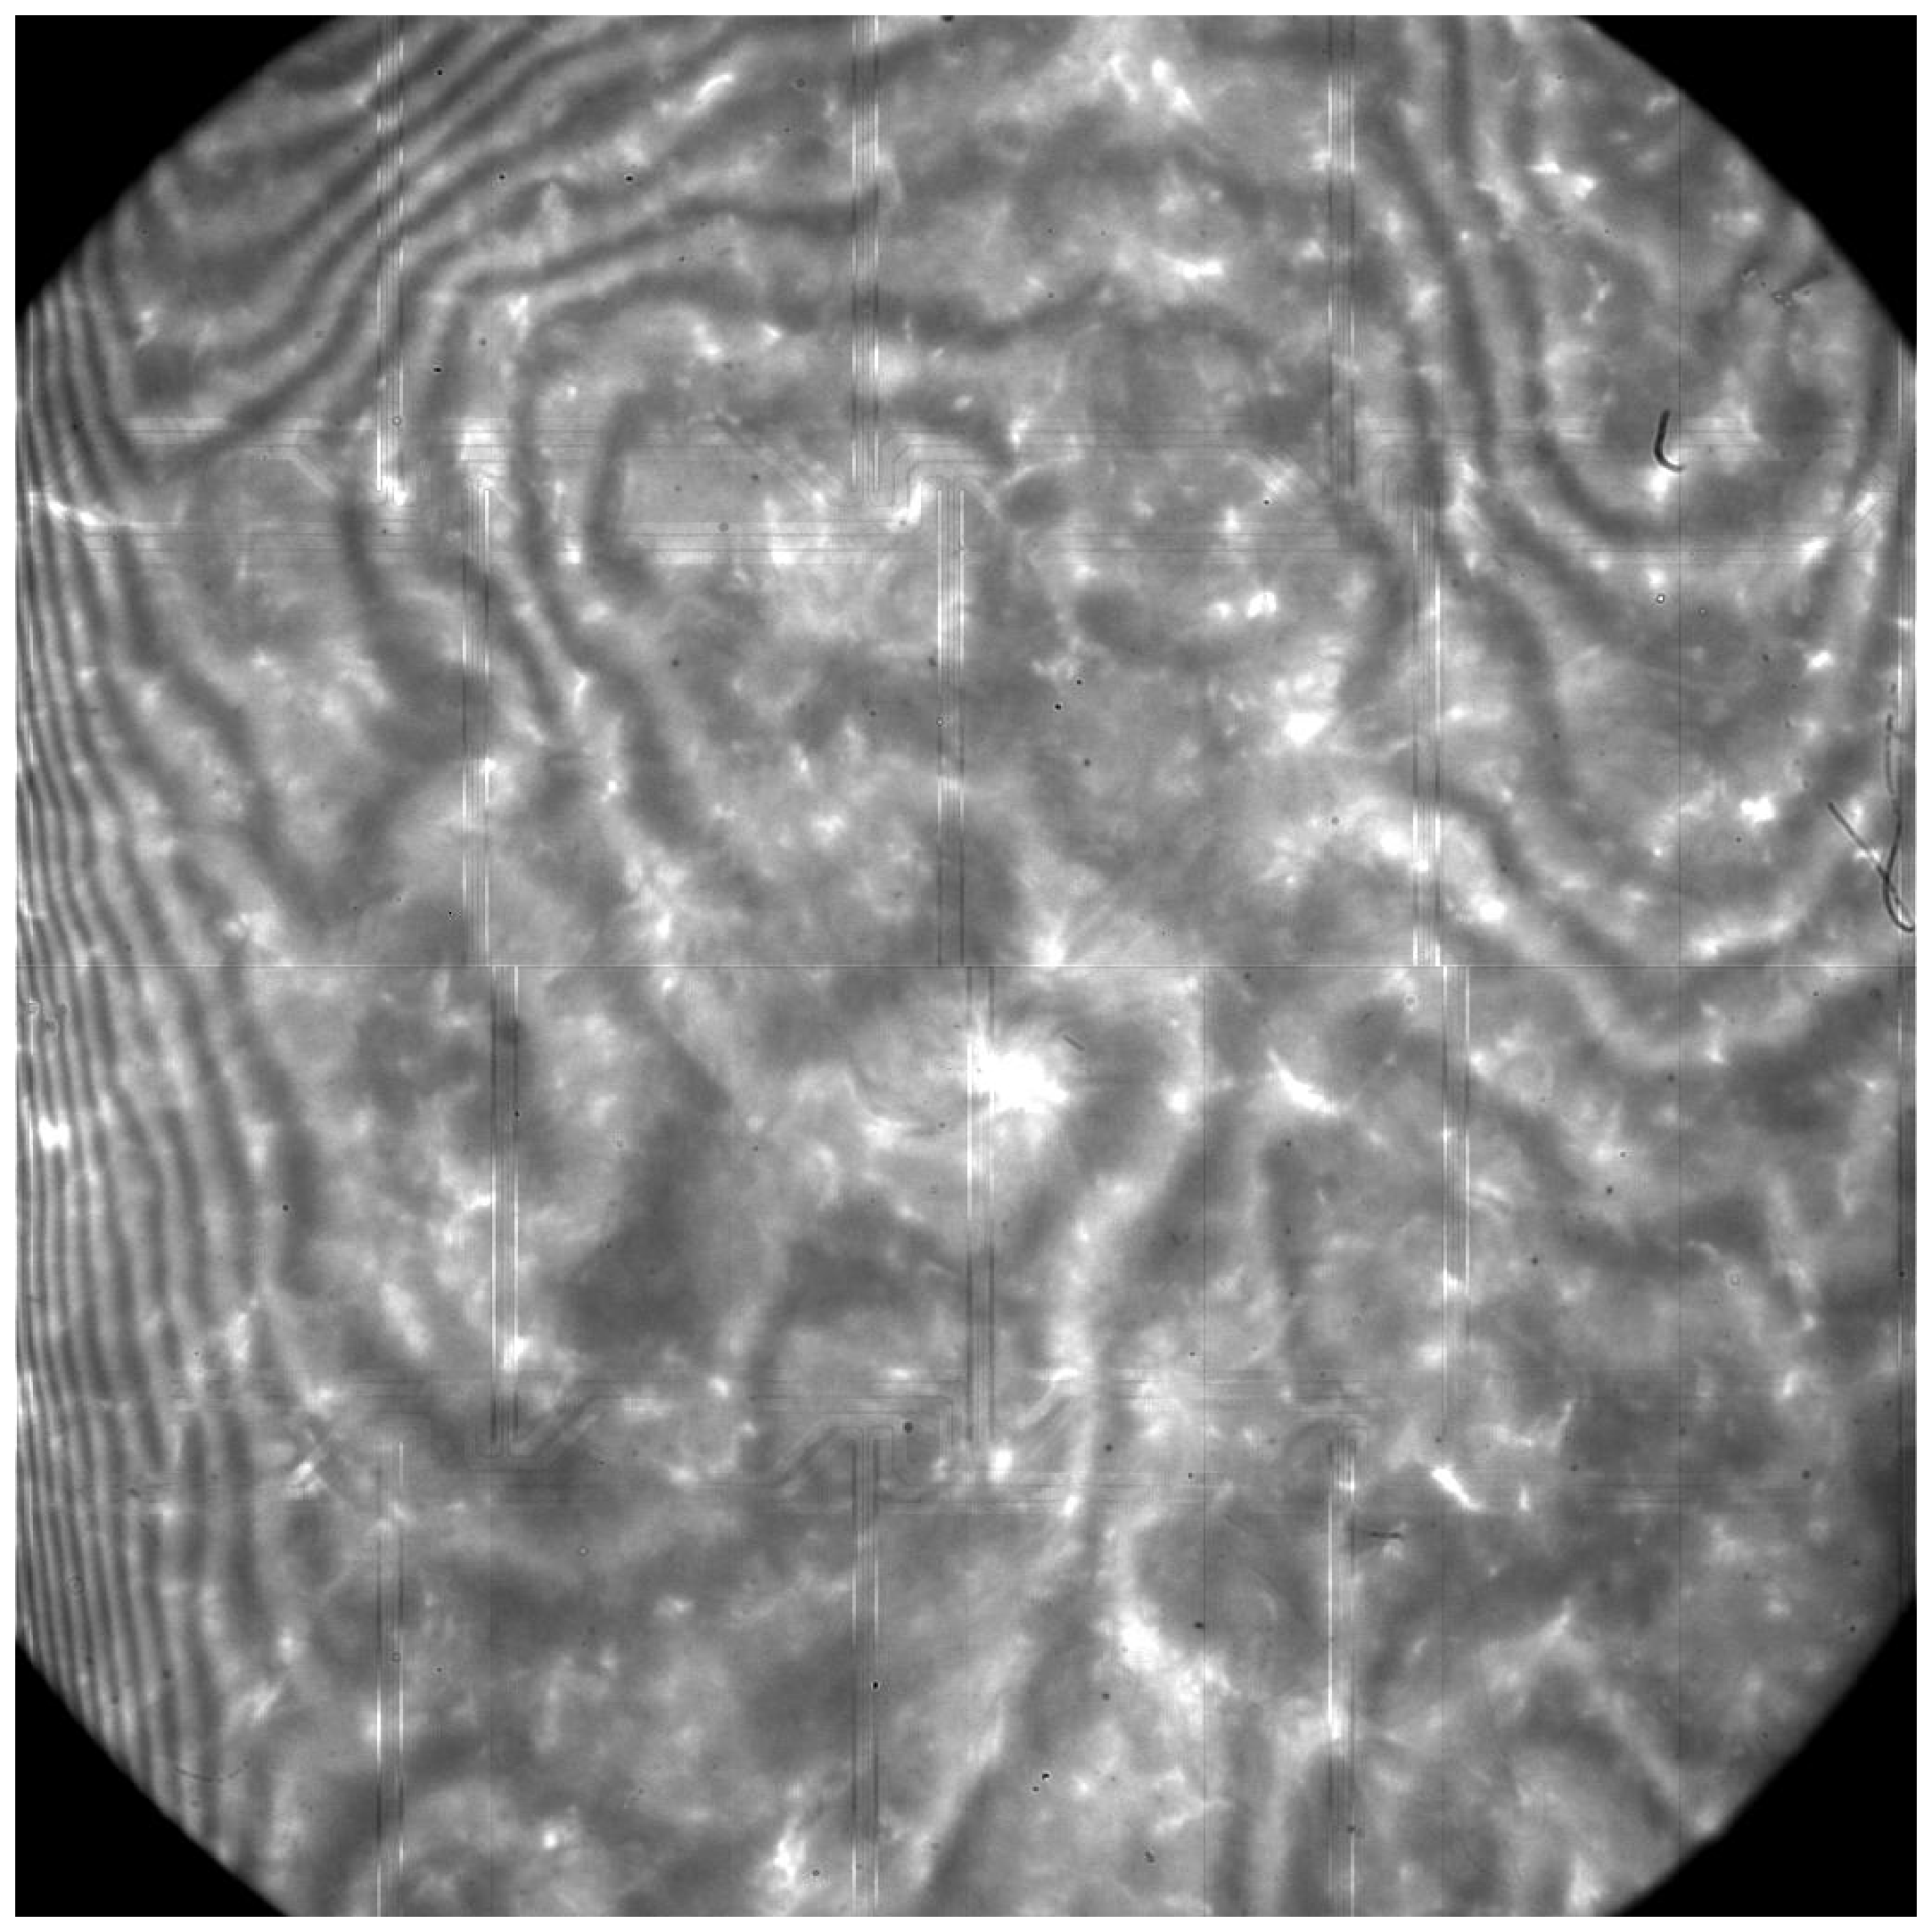
\psfig{file=camXXV_13Jun2008_8542_raw.eps,width=0.7\textwidth}
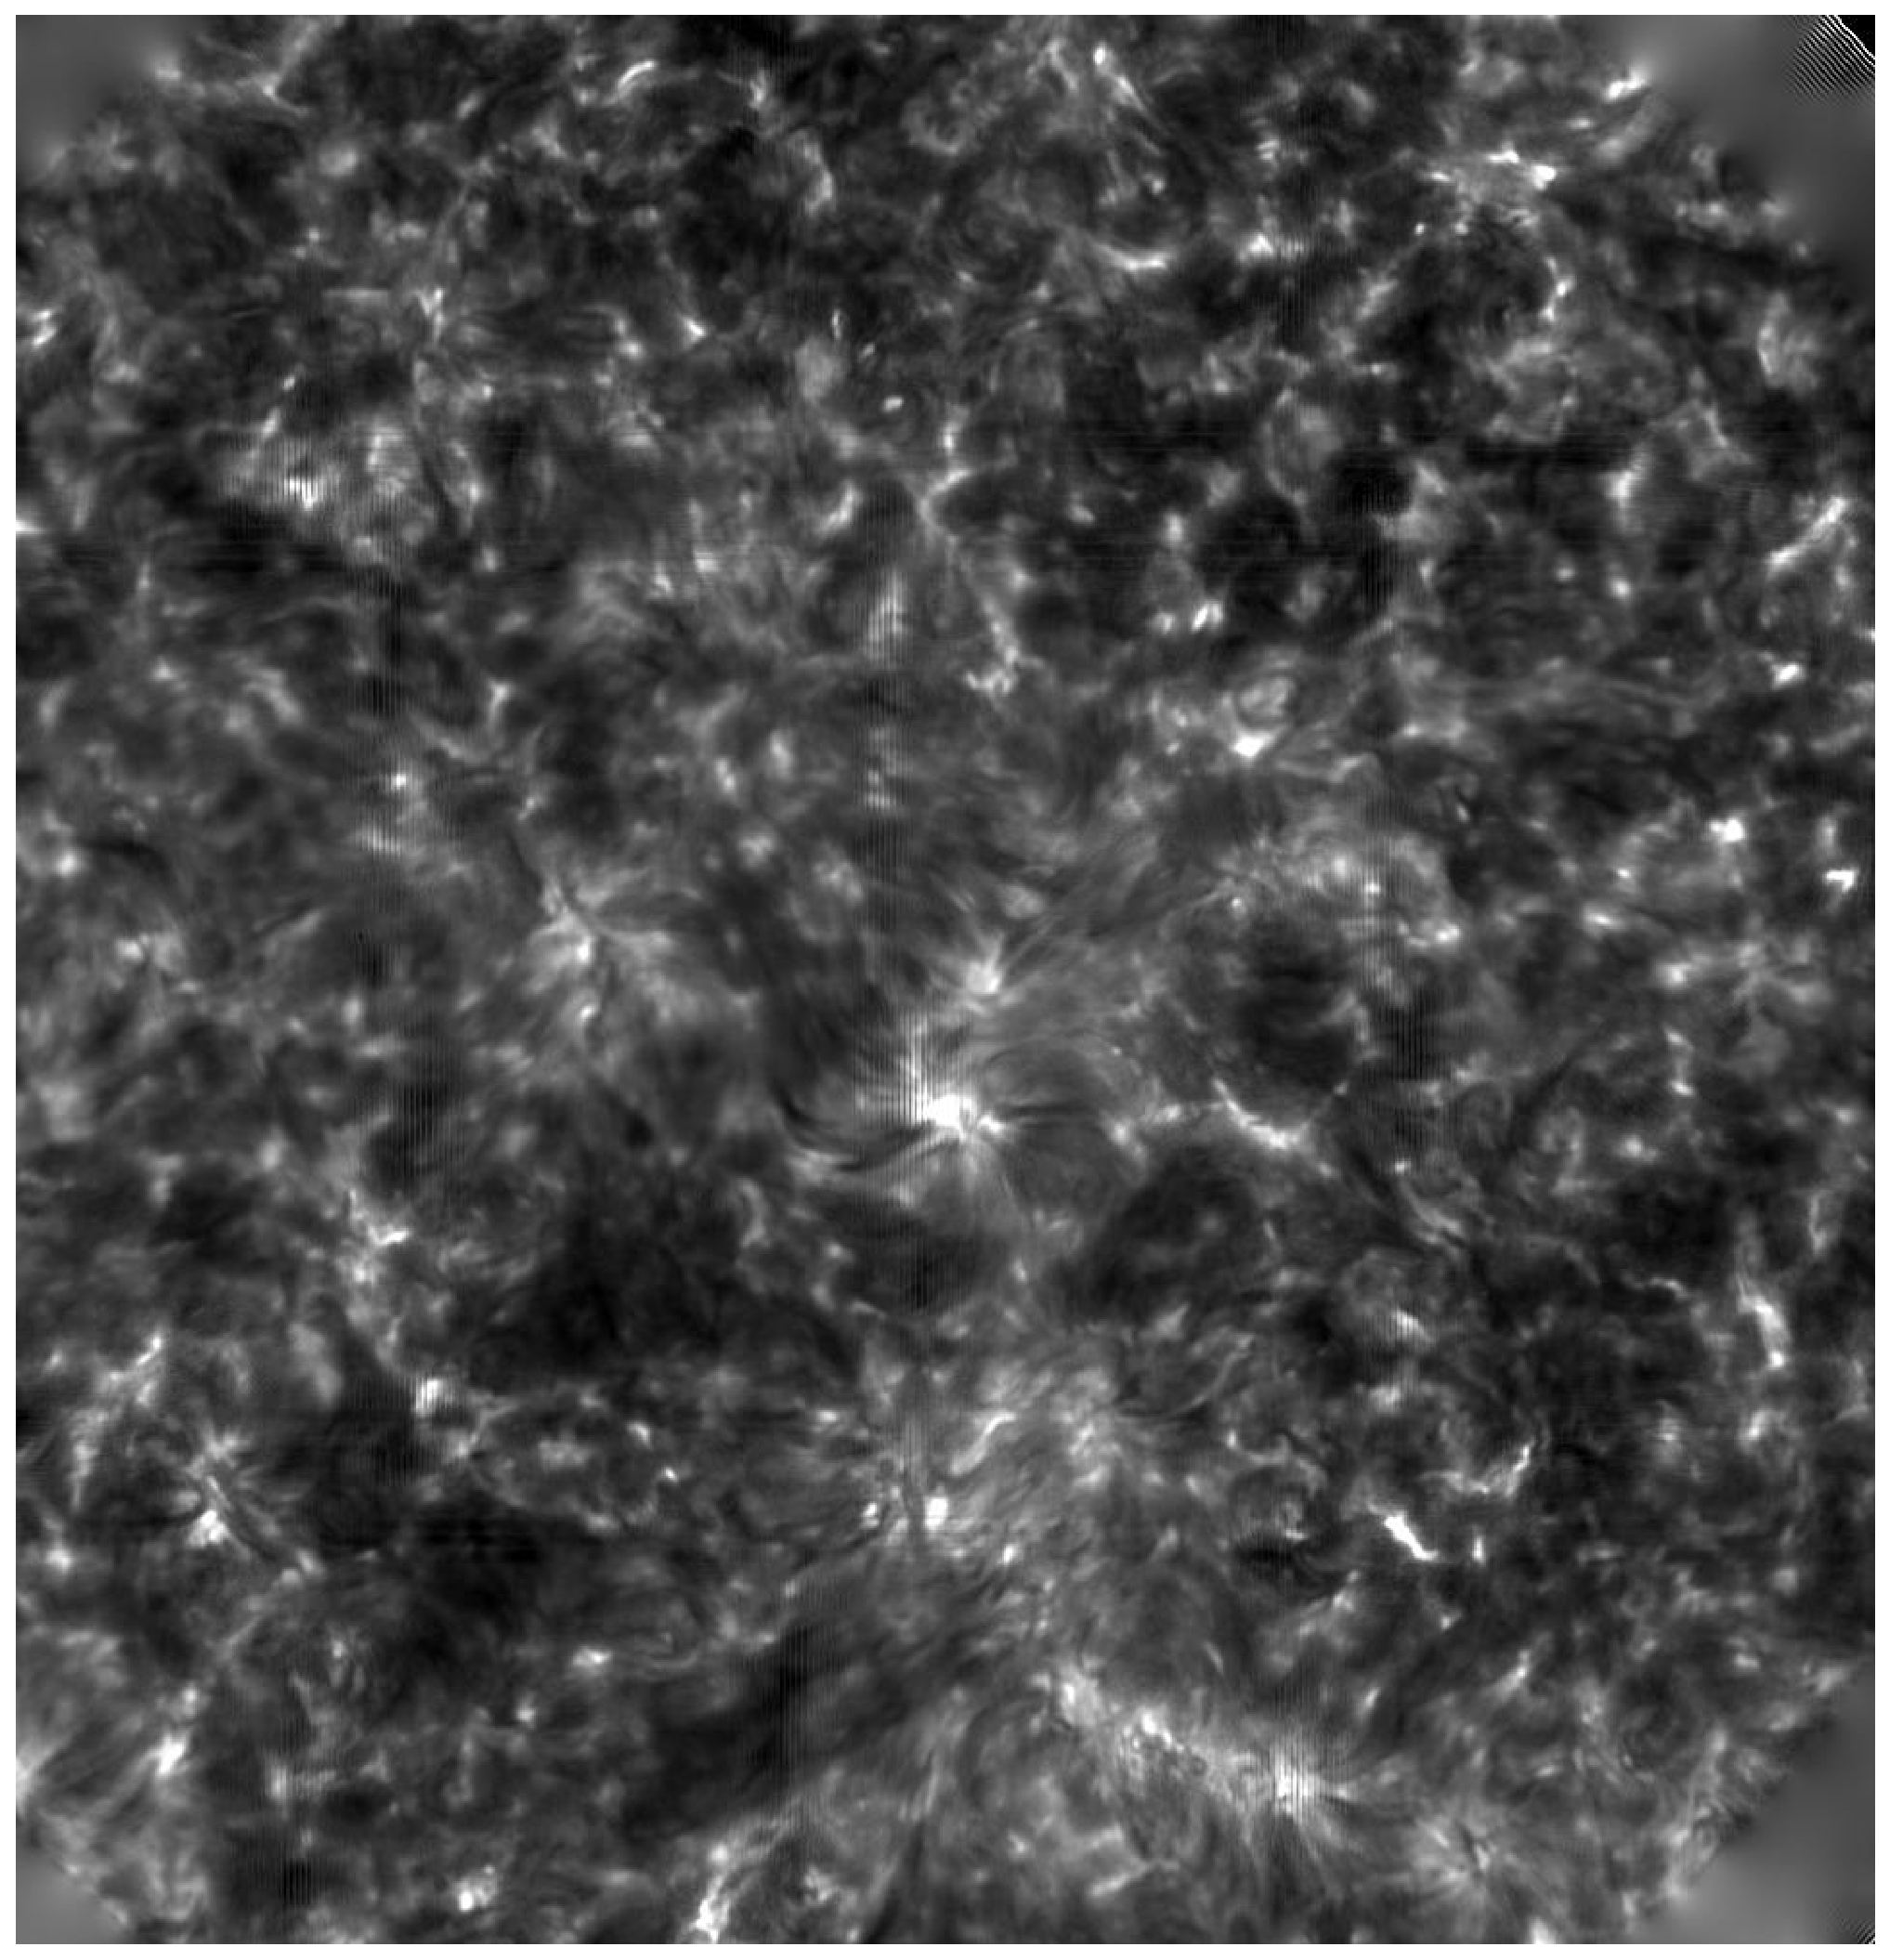
\psfig{file=camXXV_13Jun2008_8542_momfbd.eps,width=0.7\textwidth}}
\caption{Pre- and post-processed images taken of the quiet Sun in the 
$\lambda 8542$~\AA\ line of Ca~{\sc ii} at the Swedish 1-meter Solar 
Telescope, June 13, 2008 with the CRISP Fabry-Perot focal plane instrument. 
Notice that at this wavelength the CCD is partly transparent.
Notice also the patterns due fringing. Most, if not all, of these
artifacts can be removed with {\it e.g.} MOMFBD techniques.}
\label{fig:crisp8542raw-momfbd}
\end{figure}
% example from SST!

For photon energy in the range 1.14 to 3.1~eV a single electron-hole pair
is produced. At higher energies multiple electron-hole pairs will be
produced by a single photon as energetic conduction band electrons
collide with other valence band electrons. The average number of
conduction band electrons effectively generated for photon energy
$h\nu > 10$~eV is approximated by the empirical formula
\begin{equation}
  \eta = h\nu/E_{e-h}
\end{equation}
where $E_{e-h} \approx 3.65$~eV for silicon.

\subsection*{CCDs}

The CCD-detector (Charge-Coupled Device) was invented in 1969 by Boyle
and Smith at Bell Telephone Laboratory, the same laboratory where the
transistor was invented 20 years earlier. The CCD was originally
intended for use as computer memory. Its usefulness as a
electromagnetic radiation detector was, however, discovered only a few
years later. The first application of a 400$\times$400$\times 15~\mu$m
pixel CCD for high-resolution astronomical imaging was made in
1975. Since then the CCD has developed into becoming the major image
forming detector for infrared, optical and X-ray wavelengths in
astronomy as well as in other fields.  Examples include the original
800$\times$800$\times 15~\mu$m pixel detectors for the (three-phase)
Wide Field Planetary Camera (WF/PC) of the Hubble Space Telescope or
the (virtual phase) 1024$\times$1024$\times 18~\mu$m pixel detector
for the Solar X-ray Telescope of the Yohkoh Satellite. CCD detectors
are presently routinely produced in sizes 2k$\times$4k pixels, but
have also been produced in sizes up to 10000$\times$10000
pixels. Detectors of this size or larger are becoming impractical due
to rapidly increasing read-out times and production costs.

\subsection*{A simplified three-phase CCD lay-out}

The CCD depends for its functioning as a photon counting device on
four different operations: 1) the conversion of individual photons to
elementary electric charges during the illumination period, 2) the
storing of these charges over the desired exposure time, 3) the
transfer of the stored charges from pixel to pixel for the read-out
procedure, and finally 4) the accurate read-out of the accumulated
charge for each pixel element.  

In figure \ref{CCD.figschematic} a schematic lay-out for a three-phase
4$\times $5 CCD detector matrix is illustrated.  On top of a strongly
doped p-type silicon substrate is laid a weakly doped p-type epitaxial
layer, a subsequent electrically insulating SiO$_2$ layer and finally
a layer of individual transparent, poly-crystalline silicon gate
electrodes.  Each pixel element consists of three such electrodes
connected to three clocking voltage generators A, B and C. The colored
region represent the size of one pixel. Each line of pixels is
electrically separated from the neighboring lines by a strongly doped
p-implant under the oxide layer, indicated by blue lines in the
figure. The electrodes A, B and C for each pixel are electrically
connected to the similar electrode of the other pixels. In addition to
the 4$\times$5 pixel matrix the figure shows a 4 element register with
a separate set of A, B and C electrodes. The register which is
shielded from radiation is needed for the read-out process.

\begin{figure}[h]
  \centering  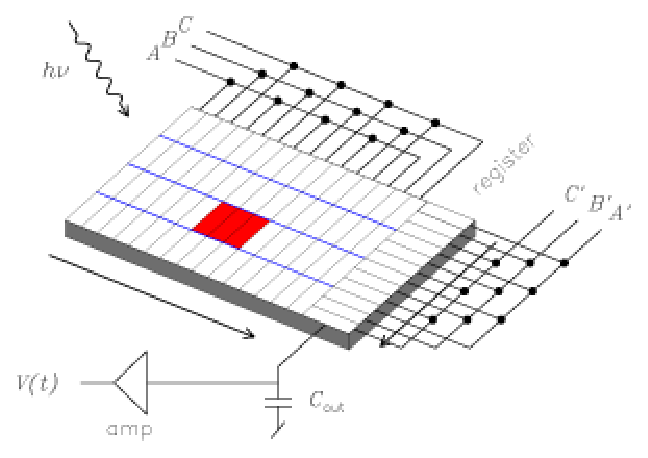
\includegraphics{CCD_schematic.eps}
  \caption{Schematic lay-out of a three-phase CCD detector}
  \label{CCD.figschematic}
\end{figure}


1) During the illumination phase the B-gate is held at high potential
(10 V) while the A- and C-gates are kept at low potential (2
V). Individual photons penetrating into the p-layer excites valence
band electrons into the conduction band. 

2) These electrons are collected in the potential well created under
the B-gate. The low potential of the A- and C-gates isolates charges
generated in any given pixel element from those generated in the
neighboring pixels.

3) The charge transfer phase is initiated by lifting C-gate to high
potential. This widens the trapping potential well and drives the
accumulated electrons towards the C-gate. This charge transport is
strengthened by subsequently lowering the potential at the B-gate. The
accumulated electrons are by now transported from under the B-gate to
under the C-gate. This procedure is next repeated twice, transporting
the electrons further on to the A- and B-gates of the subsequent pixel
element. The full procedure is then repeated until the charges
accumulated over the full length of the detector array have been
shifted out at the far end.

4) At the far end the individual shifted charge packets are dumped into
the register. Before the next set of charge packets from the different
pixels lines can be dumped to the register, the contents of the
register cells are shifted out to the measuring capacitor $C_{out}$ and
recorded by a charge measuring circuit. From the recorded
charge-versus-time series, the originating pixel element for each
charge packet can be identified and the recorded image reconstructed.

We will return to study different aspects of these different stages of
the CCD detector in greater detail below.

\subsubsection*{Other types of clocking}

Astronomical CCDs are mainly three phase devices, but there are other types
as well. 

A two phase CCD requires only a single clock, but needs double electrodes 
to provide directionality to the charge transfer process. Each pixel consistes
of two electrodes, one located deeper into the substrate than the other, 
linked to the same voltage source. Every other pixel is connected to 
alternating voltage sources. When the voltages cycle between, say, 2~V and
10~V the stored charge is attracted over to the nearer of the two neighboring
surface electrodes and then accumulates again under the buried electrode.

Virtual phase CCDs require only one set of electrodes. Additional wells with
a fixed potential are produced by p and n implants directly into the silicon
substrate. The active electrode can then be at higher and lower potentials 
as required to move the charge through the device. The active electrodes
in a virtual phase CCD are physically separated from each other leaving 
parts of the substrate directly exposed to incoming radiation. This 
enhances their sensitivity.

\subsection*{The surface channel MOS capacitor}

Let us now consider the particular silicon structure illustrated in
figure \ref{CCD.figpMOS}. On top of a heavily doped p-substrate
another weakly doped (epitaxial) p-layer with acceptor density $N_A$
is laid, then a layer of SiO$_2$ and finally a layer of
poly-crystalline silicon. The latter two layers act as an insulator and
a conductor, respectively. Note that the conducting poly-layer has
been broken up into three separate parts for each pixel for reasons to
be explained below. The dielectric constants (permitivities) of the
oxide and p-layers are $\epsilon_{ox} = 3.45 \times 10^{-11}$ F/m and
$\epsilon_{si} = 1.04\times 10^{-10}$ F/m, respectively.  The oxide
layer will prevent conduction currents to cross. The structure can
therefore be characterized as a metal-oxide-semiconductor (MOS)
capacitor.

\begin{figure}[h]
  \centering  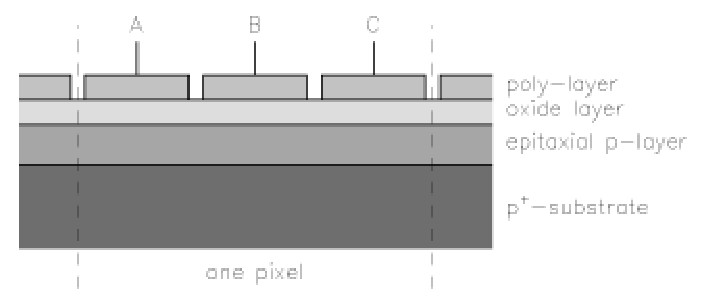
\includegraphics{CCD_pMOS.eps}
  \caption{Surface channel MOS capacitor}
  \label{CCD.figpMOS}
\end{figure}


Let the top conductive layer be given a few volts positive bias
relative to the substrate. Due to the bias voltage $V_G$ an electric
field will be established across the insulator layer and reaching a
distance $x_d$ inside the p-layer. Within this distance holes will be
swept away, leaving a region depleted of free charge carriers but with
space charge density $-e N_A$ due to the fixed acceptor ions. The
insulating layer and the depleted part of the p-layer act as two plane
parallel capacitors in series, with capacitances
\begin{equation}
  C_{ox} = \frac{\epsilon_{ox}}{d}
  \quad {\rm and} \quad C_{dep} = \frac{\epsilon_{si}}{x_d}.
\end{equation}
Inside the oxide layer a constant electric field $E_{ox}$ will be
established. Due to the existing space charge density the potential
inside the depletion region will satisfy the Poisson equation
\begin{equation}
  \dd{V}{x} = \frac{e N_A}{\epsilon_{si}}
\end{equation}
with solution
\begin{equation}
  V(x) = \frac{e N_A}{2\epsilon_{si}} (x-x_d)^2.
\end{equation}
The electric field at the oxide-silicon interface at $x=0$ is thus
given by
\begin{equation}
  E_S = -{dV\over dx}(x=0) = \frac{e N_A x_d}{\epsilon_{si}}.
\end{equation}
The discontinuity in the dielectric constant at this interface means
that there will exist a corresponding discontinuity in the electric
field. Thus (remembering that $\nabla\cdot(\epsilon{\bf E})=\rho_{free}$) 
inside the oxide layer the electric field is related to
$E_S$ through
\begin{equation}
  \epsilon_{si} E_S - \epsilon_{ox} E_{ox} = 0.
  \label{CCD.divD}
\end{equation}
The total voltage drop over the two capacitors can now be expressed in
the form
\begin{equation}
  V_G = E_{ox}d + \frac{e N_A}{2\epsilon_{si}} x_d^2,
  \label{CCD.surVG}
\end{equation}
from which an explicit expression for the thickness $x_d$ of the
depletion layer follows,
\begin{equation}
  x_d = -\frac{\epsilon_{si}}{C_{ox}} +
  \sqrt{\left(\frac{\epsilon_{si}}{C_{ox}}\right)^2
       +\frac{2\epsilon_{si}}{eN_A}\, V_G}.
  \label{CCD.xd}
\end{equation}
The result is plotted in figure \ref{CCD.figsurchan} for different
gate voltages $V_G$ for a case with uniform acceptor density $N_A =
1\times10^{21}$ m$^{-3}$.

\begin{figure}[h]
  \centering  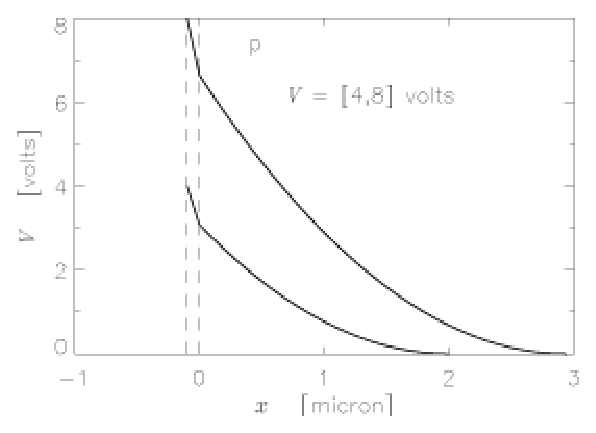
\includegraphics{CCD_surchan.eps}
  \caption{Surface channel potential well}
  \label{CCD.figsurchan}
\end{figure}


If the depletion layer is now illuminated, electron-hole pairs may be
formed. Under the influence of the existing electric field in this
region the holes will drift to the right in figure
\ref{CCD.figsurchan}. The electrons go to the left and are trapped in
the potential well at the oxide-silicon interface. If at a given time
$\tau$ during the illumination $\cl N$ electrons per unit interface
area are collected, then these represent a negative surface charge
density $\cl Q = -e\cl N$. With this surface charge present the
relation (\ref{CCD.divD}) between the electric field in the oxide layer
and the surface electric field in the depletion region must be
replaced by
\begin{equation}
  \epsilon_{si} E_S - \epsilon_{ox} E_{ox} = \cl Q
\end{equation}
When substituted in (\ref{CCD.surVG}) this means that the expression
for the thickness of the depletion region (\ref{CCD.xd}) is
transformed into
\begin{equation}
  x_d = -\frac{\epsilon_{si}}{C_{ox}} +
  \sqrt{\left(\frac{\epsilon_{si}}{C_{ox}}\right)^2+\frac{2\epsilon_{si}}{eN_A} \, V_Q},
\end{equation}
with
\begin{equation}
  V_Q = V_G + \frac{\cl Q}{C_{ox}}.
\end{equation}
Obviously, the holding capacity of the MOS capacitor for a given gate
voltage $V_G$ is exceeded when $x_d \rightarrow 0$.

\subsection*{The buried channel MOS capacitor}

The surface channel MOS capacitor studied above met with serious
difficulties in practical applications. A fraction of the accumulated
electrons tended to get trapped at imperfections at the oxide-silicon
interface. It was thus not possible to achieve the CTE values required
to build large array CCD detectors. Thus, the buried channel MOS
capacitor was invented. This structure, showing remarkable CTE
performance, differ from the corresponding surface channel structure
by having an extra n-layer (donor density $N_D$) of thickness $t$
introduced between the oxide and p-layer. The structure is
illustrated in figure~\ref{CCD.fignMOS}.

\begin{figure}[h]
  \centering  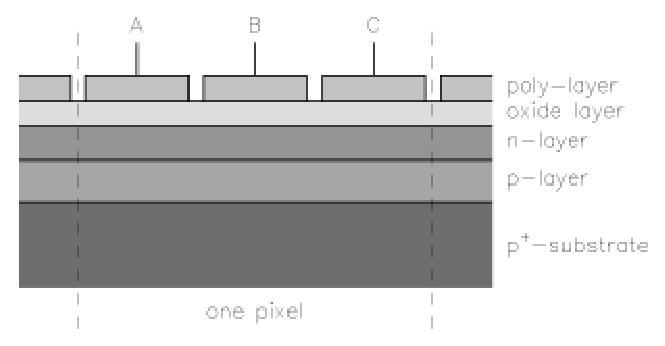
\includegraphics{CCD_nMOS.eps}
  \caption{Buried channel MOS capacitor}
  \label{CCD.fignMOS}
\end{figure}


The analysis of the buried channel MOS capacitor is only slightly more
complicated than the preceding one. The extra n-layer reshapes the
potential well to form a potential maximum between the oxide-silicon
interface and the new n-p junction. To perform as a photo-detector,
however, it is of major importance to make sure that complete
depletion of majority carriers (electrons) in the n-layer has been
achieved before the photon counting sequence is initiated. We return
to a discussion of this requirement below.

\subsubsection*{Potential well}

If we for the time being assume the depletion condition to be
satisfied the shape of the potential well is found by solving the
Poisson equation in the form
\begin{equation}
  \dd{V}{x} = \left\{ \begin{array}{ll} 
	0 & -d < x < 0 \\
	\frac{\displaystyle -eN_D}{\displaystyle \epsilon_{si}} \quad &
	0 < x < t \\
	\frac{\displaystyle eN_A}{\displaystyle\epsilon_{si}} & 
	t < x < t+x_p \\
	0 & t+x_p < x
  \end{array} \right.
  \label{CCD.Poissonbur}
\end{equation}
where $x_p$ now denotes the thickness of the p-layer depletion
region. The boundary conditions require the potential to be a
continuous function for the full $x$-range. The same applies for the
electric field $E = -\rd V/\rd x$, except at the oxide-silicon
interface where a discontinuity in the dielectric constant exits.
The solution is
\begin{equation}
  V(x) = \left\{ \begin{array}{ll} 
	V_G-E_{ox}(x+d) & -d < x < 0 \\
	V_{max} - \frac{\displaystyle
	eN_D}{\displaystyle 2\epsilon_{si}} (x-t+x_n)^2 \quad & 
	0 < x < t \\ 
	\frac{\displaystyle eN_A}{\displaystyle
	2\epsilon_{si}}(x-t-x_p)^2 & t < x < t+x_p \\
	0 & t+x_p < x 
	\end{array} \right.
  \label{CCD.bursol}
\end{equation}
where $V_{max}$ is the potential maximum occurring at a distance $x_n$
from the n-p junction. With the chosen form (\ref{CCD.bursol}) of the
solution the boundary conditions at $x = t+x_p$ is automatically satisfied.
At $x = t$ the boundary conditions dictate
\begin{eqnarray}
  N_D x_n = N_A x_p 
	\label{CCD.xn} \\
  V_{max} = \frac{eN_D}{2\epsilon_{si}}x_n^2 +
	\frac{eN_A}{2\epsilon_{si}}x_p^2.
	\label{CCD.Vmax}
\end{eqnarray}
From the requirements at $x = 0$ we find
\begin{eqnarray}
  E_{ox} = - \frac{\epsilon_{si}}{\epsilon_{ox}} \, {d{V}\over{dx}}_{(x=0^+)} \\
  V_G - E_{ox}d = V_{(x=0^+)}.
  \label{CCD.VG}
\end{eqnarray}
Finally, solving for $x_p$ we find
\begin{equation}
  x_p = -x_2+\sqrt{x_2^2+x_1^2+\frac{2\epsilon_{si}}{eN_A} \, V_G}
  \label{CCD.xp}
\end{equation}
with
\begin{equation}
  x_1^2 = \frac{N_D}{N_A}(t^2+\frac{2\epsilon_{si}}{\epsilon_{ox}}td)
  \quad {\rm and} \quad
  x_2 = t+\frac{\epsilon_{si}}{\epsilon_{ox}}d.
  \label{CCD.x12}
\end{equation}

The solution assumes uniform donor and acceptor densities $N_D$ and
$N_A$, complete depletion of the n-layer, and that the thickness $t$
and $d$ of the n- and p-layers exceeds $x_n$ and $x_p$, respectively.
In figure~\ref{CCD.figburchan} the solution is plotted for different
gate voltages $V_G$ for a case where 
$N_A = 1\times 10^{21}$~m$^{-3}$, $N_D = 1\times 10^{22}$~m$^{-3}$, 
$t = 5000$~nm, and $d = 1000$~nm.

\begin{figure}[h]
  \centering  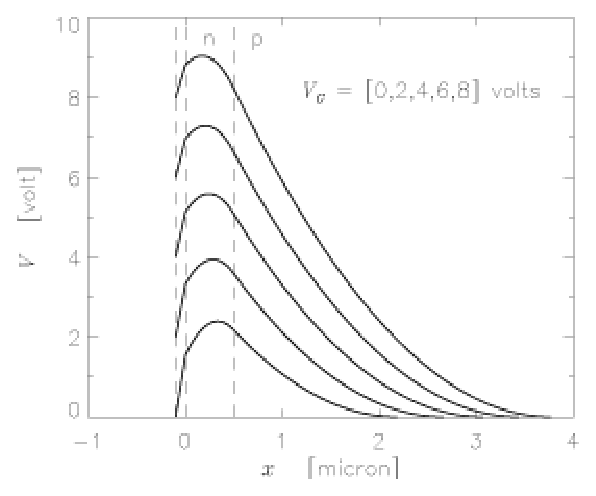
\includegraphics{CCD_burchan.eps}
  \caption{Buried channel potential well}
  \label{CCD.figburchan}
\end{figure}


\subsubsection*{Depletion}

At the n-p junction mobile carriers from both sides (electrons form
the n-side and holes from the p-side) will tend to diffuse across the
junction and recombine with the opposite type carriers from the other
side. In this way a region on both sides of the junction will be
depleted of carriers, but with space charge densities determined by
the dopant concentrations, $N_D$ and $N_A$, respectively. Left to
itself a contact potential of approximately 0.7 V will be established
across the n-p junction, creating an electric field directed from the
n-side to the p-side and of sufficient strength to stop further
diffusion of carriers across the junction\footnote{There are in fact
  small currents, even in equilbrium, but in that case they are equal
  such that $I_{\rm r}=I_{\rm g}$. The first {\it recombination
    current}, $I_{\rm r}$ is due to the majority carriers that are
  able to overcome the potential barrier $V_{\rm b}$, cross the
  depletion barrier, and undergo recombination. $I_{\rm r}$ has two
  components; one caused by n-side electrons, the other by p-side
  holes. The magnitude of this current will depend on the temperature
  and on the size of the barrier. The second {\it generation current},
  $I_{\rm g}$, is due minority carriers and flows in the opposite
  direction. The minority carriers are thermally ionized
  conduction-band electrons on the p-side and valence band holes on
  the n-side, which defuse away from their creation sites. If they
  reach the depletion region, they will be swept across. Diffusion
  speed outside the depletion region will depend on the temperature
  and the impurity concentration, but $I_{\rm g}$ is independent of $V_{\rm b}$}.

A potential bias applied across the n-p junction will disturb this
equilibrium. For a forward bias, acting to reduce the self-generated
electric fields at the junction, the diffusion of majority carriers
from both sides will continue and an electric current will flow across
the junction. For a reverse bias the self-generated electric field
will be strengthened, driving majority carriers on both sides further
away from the junction and increasing the width of the depletion
region.

An analysis similar to the one above will show that the widths of the
depletion layers, $x_n$ and $x_p$, on the two sides of the junction
are given by
\begin{equation}
  x_n = \frac{N_A}{N_D} \, x_p,
 \label{eq:npjunction1}
\end{equation}
with
\begin{equation}
  x_p = \sqrt{\frac{2\epsilon_{si} N_D}{eN_A(N_A+N_D)} \, V_{\rm ref}}. 
 \label{eq:npjunction2}
\end{equation}
The situation is illustrated in figure \ref{CCD.figjunction}.

\begin{figure}[h]
  \centering  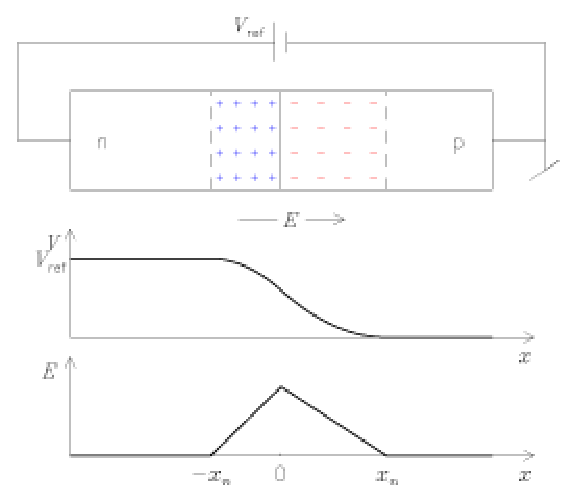
\includegraphics{CCD_junction.eps}
  \caption{n-p junction depletion region}
  \label{CCD.figjunction}
\end{figure}

Similarly, with the n-channel potential lying above the gate
potential, the electric field near the oxide-silicon interface will
drive n-channel majority carriers away from this interface. This
creates another depletion region starting from the oxide-silicon
interface. With increasing $V_{ref}$ (the potential of the non-depleted
and therefore conducting part of the n-channel) relative to the gate
potential $V_G$, the width of the gate-induced depletion region
increases. Eventually, the two depletion regions from the n-p junction
and the oxide-silicon interface grow together. This occurs when
$V_{max} = V_{ref}$. At this point the voltage generator supplying the
$V_{ref}$ bias to the n-channel will lose control. The n-channel is
no longer conducting and the gate potential $V_G$ will take control
and govern the subsequent process. This is also the necessary
initialization requirement for the buried channel CCD to work as a
photo-detector.

The n-p junction described above is an example of a diode: it will
carry positive current in the direction p to n, but not in the reverse
direction. The size of the current will depend on the potential
$V_{\rm ext}$ applied over the diode.
Absorption of a photon in a diode causes an ionization and
the creation of a conduction band electron and valcence bond
hole. This adds a new contribution to the generation current dependent
on $\phi$, the number of photons that enter the detector per
second. The total current will then be something like
\[
I_{T}=-q\phi\eta+I_{\rm r}+I_{\rm g}
\]
where $\eta$ is a factor that depends on the fraction of incident
photons that are absorbed as well as the probability that a generated
charge carrier will cross the junction before
recombining. Electron-hole pairs created in the depletion zone are
immediately swept apart by the strong electric field there, while
those created outside must first diffuse to the diffusion zone and can
therefore recombine before reaching that far. 

A light sensitive diode can be used in several ways:
\begin{itemize}
\item As a {\it photo-conductor} where a battery holds the external voltage
  to a constant value and the current is a linear function of the
  incident photon flux.
\item As a {\it power-cell} the diode is connected to a constant-load
  resistance, and the power output depends on the incident photon
  flux. This is the principle behind solar power cells.
\item In the {\it photovoltaic} mode current from from the diode
  is held at zero, making it a stroage capicitor, and the voltage
  across it is a non-linear function of the photon flux.
\end{itemize}

\subsubsection*{Storage capacity}

As the CCD detector is subsequently illuminated, the generated
photoelectrons will be collected in a region around the maximum
potential $V_{max}$ in the n-channel. This region therefore becomes
non-depleted, with part of the space charge density of the donor ions
neutralized by the photo-electron space charge density. This in turn
means that the potential maximum starts to decrease and the charge
collection region to widen. 

Indeed, we expect a flat-topped potential distribution within the
photo-electron collection region. Due to the presence of the
photo-electrons, this region will be electrically conducting and where
the internal electric field and the net space charge density
from donor ions and photo-electrons both vanish. The width $\Delta x$
of the flat-topped potential part is therefore determined by the
relation
\begin{equation}
  \Delta x = -\frac{\cl N}{N_D},
\end{equation}
where $\cl N$ is the collected number of photo-electrons per unit
detector area.

The analysis of the buried channel MOS capacitor with photo-electrons
present is rather similar to the one carried out above. The Poisson
equation now reads
\begin{equation}
  \dd{V}{x} = \left\{ \begin{array}{ll} 
	0 & -d < x < 0 \\
	\frac{\displaystyle -eN_D}{\displaystyle \epsilon_{si}} \quad &
	0 < x < t-\Delta x -x_n \\
	0 & t-\Delta x -x_n < x < t -x_n \\
	\frac{\displaystyle -eN_D}{\displaystyle \epsilon_{si}} \quad &
	t-x_n < x < t \\
	\frac{\displaystyle eN_A}{\displaystyle\epsilon_{si}} & 
	t < x < t+x_p \\
	0 & t+x_p < x
  \end{array} \right.
  \label{CCD/.Poissonburph}
\end{equation}
with solution
\begin{equation}
  V(x) = \left\{ \begin{array}{ll} 
	V_G-E_{ox}(x+d) & -d < x < 0 \\
	V_{max} - \frac{\displaystyle
	eN_D}{\displaystyle 2\epsilon_{si}} (x-t+\Delta x +x_n)^2 \quad & 
	0 < x < t-\Delta x - x_n \\ 
	V_{max} & t-\Delta x - n_n < x < t - x_n \\
	V_{max} - \frac{\displaystyle
	eN_D}{\displaystyle 2\epsilon_{si}} (x-t+x_n)^2 \quad & 
	t - x_n < x < t \\ 
	\frac{\displaystyle eN_A}{\displaystyle
	2\epsilon_{si}}(x-t-x_p)^2 & t < x < t+x_p \\
	0 & t+x_p < x.
	\end{array} \right.
\end{equation}
The boundary conditions (\ref{CCD.xn})-(\ref{CCD.VG}) are still
valid. We note that the given form of the solution ensures that the
boundary conditions at the borders of the charge collection region are
automatically satisfied. The solution (\ref{CCD.xp}) is still
valid, but the definitions of $x_1$ and $x_2$ in (\ref{CCD.x12}) have
to be replaced by
\begin{equation}
  x_1^2 = \frac{N_D}{N_A}\left[(t-\Delta
  x)^2+\frac{2\epsilon_{si}}{\epsilon_{ox}}(t-\Delta x)d \right] 
  \quad {\rm and} \quad
  x_2 = t-\Delta x+\frac{\epsilon_{si}}{\epsilon_{ox}}d.
  \label{CCD.x12ph}
\end{equation}

In figure \ref{CCD.figburchanph} the potential structure for a given
gate voltage $V_G$, but for different values $\cl N$ of collected
photo-electrons per unit detector area is given. The parameters for
the MOS capacitor are identical to that of figure~\ref{CCD.figburchan}. 
With $\cl N = 15\times 10^{14}$ m$^{-2}$ the
charged region is less than 40~nm away from the oxide-silicon
interface.

We conclude that there will exist an upper limit to how much charge
can be stored in the device. An over exposure of one pixel element
will mean that surplus photo-electrons will start to leak into
neighboring pixels, producing a ``blooming'' effect in the image.


\begin{figure}[h]
  \centering  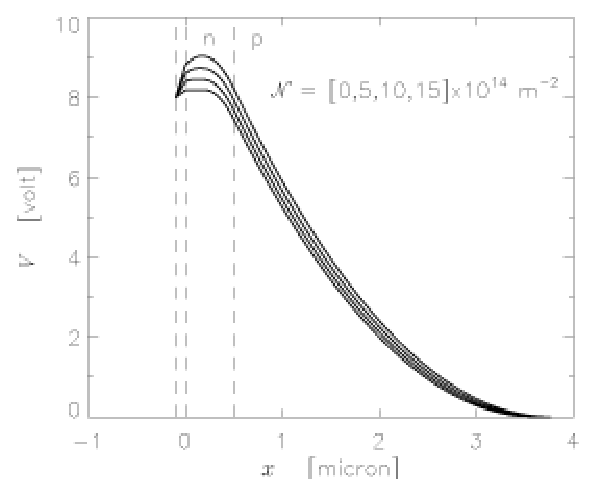
\includegraphics{CCD_burchanph.eps}
  \caption{Buried channel potential structure with photo-electrons present}
  \label{CCD.figburchanph}
\end{figure}




\subsection*{The charge transfer process} 

After the illuminated charge generation phase the collected charges
need to be transfered to a suitable charge measuring circuitry. In a
three-phase CCD array each pixel is supplied with three separate gate
electrodes as illustrated in figures~\ref{CCD.figpMOS} or
\ref{CCD.fignMOS}, each of these electrodes are connected with the
corresponding electrodes of the neighboring pixels.  In the
collecting phase the middle electrode of each pixel is biased high (10
V), the others low (2 V). Photo-electrons generated over the full pixel
will collect in the potential well existing under the B electrode.
Electrodes A and C act to isolate charges generated in the selected
pixel from similar charges generated in the neighboring pixels.

At the end of the illumination period the charge transfer phase
starts. This is done by applying clocking potentials to the gate
electrodes as indicated in figure~\ref{CCD.figclocking}. The transfer
of electrons from B to C starts by raising the gate electrode C to
high potential. This will widen the potential well under gate B to
also include gate C. The collected electrons will drift to fill the
widened potential well uniformly due to self-induced repulsion. Next
the B-gate potential is lowered, creating fringing fields that push
the remaining electrons under B toward C. In this way the electrons
have been shifted one gate position and are ready to be shifted to
gate A of the next pixel and so on. After three gate shifts the
collected electrons have been moved one pixel.

Optimum performance of the transfer process is achieved for slow slew
rates of the clocking signals. The characteristic RC rise and fall times
 $\tau_{RC}$ of the clocks are therefore often related to the one pixel
transfer time $t_T$ by
\begin{equation}
  \tau_{RC} = \frac{t_T}{12}.
\end{equation}
This is the choice made in figure~\ref{CCD.figclocking}. A typical
value of the transfer time may be $t_T = 1$ $\mu$s.

\begin{figure}[h]
  \centering  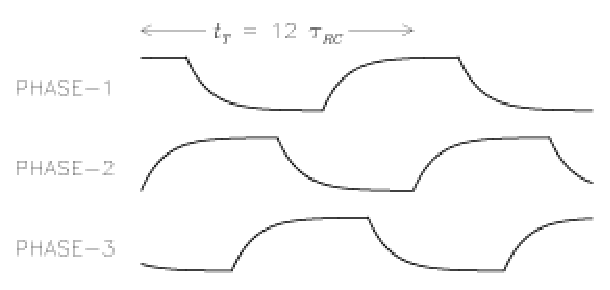
\includegraphics{CCD_clocking.eps}
  \caption{Clocking signal for three-phase CCD}
  \label{CCD.figclocking}
\end{figure}


\subsection*{Charge measurements} 

The final operational phase of the CCD detector is the measurement of
the charges accumulated in the different pixels during the exposure
time. This is accomplished by dumping the transfered charges on to a
small capacitor connected to a MOSFET amplifier. The MOSFET amplifier
is the only active element of the CCD detector, that is, it is the
only element that requires power. The individual pixel elements made
up of MOS capacitors are themselves passive elements.

The output amplifier generates a voltage proportional to the charge
transfered, the larger voltages the smaller the capacitance of the
output capacitor. Important engineering design criteria for the output
stage is to minimize the noise generation in the MOSFET
amplifier. This can be achieved by cooling the CCD detector to
temperatures down to about - 90$^\circ$C.  Modern
high-performance CCDs have achieved remarkable noise level
equivalents down to less than 2 (elementary) electron charges.

\subsection*{Dark currents}

Operating the CCD detector under reduced temperatures will also reduce
problems related to dark currents in the MOS capacitors. The basic
underlying assumption of the CCD as a photon counting device is that
the photoelectrons are the only source of the accumulated charge. This
assumption is challenged by the existence of dark currents. Dark
currents occur naturally in semiconductors through thermal generation
of charge carriers. Dark current generation occurs independent of the
illumination state of the semiconductor, thus its name. The only way
of reducing this error source for a given detector is to lower the
operating temperature. The dark current level for a given temperature
is, however, strongly dependent on the fabrication process and the
quality of the silicon used in the production.

There are three main regions that contribute to dark currents: the
neutral bulk material below the potential well, the depleted material
within the potential well and the oxide-silicon interface. Normally
the latter is the more important one. Dark current carriers are
generated through the presence of midband energy states halfway
between the valence and conduction bands. These states are associated
with imperfections or impurities within the semiconductor or at the
oxide-semiconductor interface. They promote dark currents by acting as
stepping stones for two-step thermal transitions of electrons and
holes between the valence and conduction bands. Any electron raised to
the conduction band through this process in the depleted region will
be collected in the potential well together with the desired
photoelectrons. Corresponding electrons generated in the field-free
region outside the depletion region may enter this region through a
diffusion process, then to be collected by the existing electric field.
 
The temperature variation of the dark current in the CCD is well
described by the formula
\begin{equation}
  I_d = C \cl T^{3/2} \exp(-U_g/\cl T),
\end{equation}
where $C$ is a constant for each detector and $U_g$ is the silicon
band-gap energy. The band-gap energy is found to follow the empirical
formula (in eV units)
\begin{equation}
  U_g = 1.1557 - \frac{7.021\times 10^{-4}\, T^2}{1108+T}
\end{equation} 
with temperature $T$ given in degrees K. In figure \ref{CCD.figdark}
the dark current for the CCD normalized to unity for room temperature
($T = 300$ K) is plotted.  One should bear in mind that the operating
temperature of the CCD cannot be made arbitrarily low. To function the
temperature of the CCD must be high enough that the dopant atoms
remain in ionized state in the lattice and thus contribute to the
formation of potential wells. This requires operating temperatures
exceeding 70 K.

\begin{figure}[h]
  \centering  \includegraphics{CCD_dark.eps}
  \caption{Normalized dark current as a function of temperature }
  \label{CCD.figdark}
\end{figure}

\subsection*{CCD summary, problems and corrections}

For typical noise levels and pixel capacities, astronomical CCDs have dynamic
ranges of $100\,000$ to $500\,000$.

A major problem is the noise produced by cosmic rays. A single cosmic ray
particle coming through one of the pixels of the detector can cause a large
number of ionizations. The resulting electrons accumulate in the storage 
region along with those produced by photons. These are usually recognizable
by the observer as `spikes' in the image. Replacing such spikes is possible
by using the average of the surrounding pixels, but this does not retrieve 
the original information lost. In addition the correction must often be done
`by hand' which can be time consuming. Automatic removal of spikes is 
sometimes possible given several individual images of the same object or a 
good model of the data --- but such automatic removal is difficult and 
can become a `black art'. 

Another defect of CCDs is the variation in the background noise between 
pixels. There may be large-scale variations of 10--20~\% over the whole
sensitive area, and there may be individual pixels with permanent high levels.
The first problem can be reduced by flat fielding if its effect can be 
determined by observing a uniform source. The effect of a single hot spot
may also be reduced in signal processing by replacing it with an average of
its neighbors. However, the hot spot pixel is often also a poor transporter 
of charge resulting in a spurious line being introduced into the image.

Yet another problem is that of cross talk or blooming. This occurs when 
electrons stray to nearby pixels. This especially effects rear illuminated 
CCDs as in them electrons are produced quite far from the electrodes. This
is the reason rear illuminated CCDs are thinned; {\it ie} to reduce this 
distance. It will also occur for any CCD where the accumulating charge nears
its maximum capacity. 

\subsection*{Other types of detectors}

In these notes we have concentrated almost exclusively on CCD's, but one should
be aware that also other types of detectors exist. These are covered were
summarily here and in somewhat more detail in chapter~1 of Kitchin's 
{\it Astrophysical Techniques}.

\subsubsection*{Photomultiplyers}

Electron photomultiplyer phototubes were once the workhorse of optical 
astronomy. They continue to be used when individual photons need to be
detected  as in neutrino and cosmic ray \^Cerenkov detectors or when very
rapid responses are required as in observations of occultations.

Photomultiplyers detect photons through the photoelectric effect. A 
photoemitter is coated on to the cathode and this is at a negative potential
of some 1000~V. Once a photoelectron has escaped from the photoemitter, it
is accelerated by an electric potential until it strikes a second 
electron emitter. The primary electron's energy then goes into pair production
and secondary electrons are emitted from the substance in a manner analogous
to photo-electron emission. Several secondary electron emissions result 
from a single primary electron. The secondary emitter is coated onto dynodes
that are successively more positive than the cathode by 100~V or so for each
stage. The various electrodes are shaped and positioned so that the electrons
are channelled towards the correct next electrode in the sequence after 
each interaction. The final signal pulse may contain $10^6$ electrons for each
incoming photon. 

\subsubsection*{Superconducting tunnel junction detectors (STJs)}

Kitchin mentions that a possible replacement of CCDs could come in the form
of superconducting tullel junction detectors (STJ). At temperatures
below $T_{\rm c}$, an unlimited number fo superconducting states exist
at an energy $\Delta$ below the Fermi level. Single electrons will
therefore occupy only states of energy $(E_{\rm F}-\Delta$ or
  lower. $\Delta$ is a strong function of temperature rising from zero
  at $T_{\rm c}$ to a maximum $\Delta_{\rm m}$ at temperatures below
  about $0.3T_{\rm c}$. The value of $\Delta_{\rm m}$ measures the
  binding energy per electron of a {\it Cooper pair} is very small;
  for example $1.4\times 10^{-4}$~eV for Pb, which is typical. If a
  superconductor is to absorb a photon it must have energy larger than
  $2\Delta$ so that a Cooper pair can be broken up and both electrons
  promoted to excited states in the ``conduction'' band. These
  electrons will have quantum characteristics that differ from
  energetic electrons in an ordinary metal, and are therefore termed
  {\it quasiparticles}. The number of states available to
  quasiparticles at energies just above the gap is very large.

The STJ can operate 
from the UV to the longwave infrared, and also in the X-ray region.
Its operating principle is based on a {\it Josephsons junction}. This has two 
superconducting layers separated by a insulating layer that is thin
enough (of order 1~nm) to permit quantum mechanical tunneling. A
junction can be arranged as a light-detecting diode by applying a
positive bias voltage less than $V^{+}=2\Delta/q$ to one of the
superconductors and a magnetic field applied parallell to the
junction. If the junction is very cold all excited states are
empty. In a normal Josephson junction Cooper pairs could tunnel across
the insulating layer to the superconductor with applied voltage
$V^{+}$, but the applied magnetic field hindres this, and the diode
does not conduct.

If the superconductor without applied voltage absorbs a photon of
energy $hc/\lambda$ it receives enough energy to break apart mulitple
Cooper pairs, promoting a maximum of $hc/\lambda\Delta$ electrons into
excited states. These quasiparticles {\it can} tunnel across the
insulator, and those that do produce a current pulse that is inversely
proportional to the wavelength $\lambda$ of the exciting photon.

The STJ detector can therefore count individual incoming photons and
determine their wavelength, from X-ray to infrared, of each. This is a
technology still in development, but some practical multi-pixel
STJ-based detectors have begun to appear at telescopes.

\subsubsection*{Other types}

\noindent{\it Photvoltaic cells.} These are also known as photodiodes,
photoconductors, and barrier junction detectors. The idea is to use the
properties of a p-n junction in a semiconductor. When such a junction
is in equilibrium electrons and holes have diffused across the
junction until a sufficient potential difference is set up to halt the
flow. The two Fermi levels are then coincident and the potential
across the junction is equal to their original difference. If now
light falls on the junction it can generate electron-hole pairs in
both the n-type and the p-type materials. The electrons in the
conduction band of the p-region will be attracted towards the n region
by the intrinsic potential difference across the junction, and they
will be free to flow in that direction. The holes in the valence band
of the p-type material will be opposed by the potential and will not
move. In the n-type region the electrons will be similarly trapped
while the holes will be pushed across the junction. Thus a current is
generated by the illuminating radiation and this may simply be
monitored and used as a measure of light intensity. For use as a
radiation detector the p-n junction often has a region of undoped (or
intrinsic) material between the p and n regions in order to increase
the size of the detecting area. These devices are known as p-i-n
junctions, and their operating principle does not differ fro that of
the simple p-n junction.

\noindent{\it Thermocouples.} Two dissimilar metals in contact can
develop a potential difference across their junction. This is called
the Seebeck effect. The position of the Fermi level will change with
temperature and the change in Fermi level may not be the same in two
dissimilar metals, and so at the junction the difference between the
two Fermi levels will vary with temperature. In a thermocouple, two
dissimilar metals are joined into a circuit that incorporates a
galvanometer. When one junction is at a different temperature from the
other, their Seebeck potentials differ and a current flows through the
circuit. 

A practical thermocouple for radiation detection is made from two
metals in the form of wires that are twisted together and blackened to
improve their absorption. The other junction is kept in contact with
something with a large thermal inertia so that it is kept at a
constant temperature. Several thermocouples are usually connected
serially so that their potentials combine. This is called a {\it
  thermopile}.

Practical thermocouples and thermopiles are usually made from antimony
and bismuth or from nickel and various mixtures of copper, silicon,
chromium, aluminium etc. They are useful wide-band detectors,
especially for infrared work. Their simplicity of operation and
robustness has led to many application for them despite their
relatively low sensitivity.

\noindent{\it Phototransistors.} These are of little direct use in
astronomy because of their low sensitivity. They consist simply of a
p-n-p or n-p-n transistor with the minority current carriers produced
by the illumination instead of the normal emitter. Thus the current
rises with increasing radiation and provides a measure of its intensity.

\noindent{\it Charge injection devices} (CID) -- detection method identical to CCD, 
the difference lies in the read out system. 

\subsubsection*{Infrared detectors}

Many of the detectors mentioned above have some infrared (IR) sensitivity, 
especially out to 1~$\mu$m. At longer wavelengths, other types of detectors
are needed. The IR region is conventionally divided into three: the near
(NIR), 0.7--5~$\mu$m, the mid (MIR), 5--30~$\mu$m and the far (FIR), 
30--1000~$\mu$m. All IR detectors need to be cooled, with the longer the
operating wavelength, the colder the required temperature. Thus in the 
NIR liquid nitrogen (77~K) suffices, in the MIR liquid helium (4~K) is 
needed, while one must operate at temperatures down to some 100~mK in the 
FIR. Currently there are two types of detector in the IR: the photoconductor
of the NIR and MIR (and somewhat into the FIR) and the bolometer for the
FIR.

\noindent{\it Photoconductive cells} exhibit a change in conductivity with the 
intensity of their illumination. The mechanism for that change is the 
absorption of radiation by the electrons in the valence band of a 
semi-conductor and their consequent elevation to the conduction band. The
conductivity therefor increases with increasing illumination, and is monitored
by a small bias current. These cells have been assembled into arrays of 
up to $2048\times 2048$ for the NIR and $1024\times 1024$ for the MIR, 
though at the long wavelength end of the MIR arrays of some hundred cells is
the maximum. In the FIR sizes are still only up to $32\times 32$. Unlike
CCDs infrared arrays are read out pixel by pixel. 

\noindent{\it Bolometers} are devices that change their electrical
resistivity in response to heating by illuminating radiation. At the
simplest, two strips of material are used as the arms of a Wheatstone
bridge. When one is heated by the radiation its resitance changes and
so the balance of the bridge alters. 

\subsection*{Noise}

In the absence of noise any detector would be capable of detecting any source,
however faint. A minimum signal to noise ratio of unity is required for 
detection. However, most research work requires signal to noise ratios of
at least 10, and preferably 100 or 1000. 

Noise sources can be separated into four classes: {\it intrinsic noise} 
originating from the detector, {\it signal noise} arising from the character
of the of the incoming signal, {\it external noise} e.g. spurious signals
from cosmic rays and the like, {\it processing noise} from amplifiers and
similar used to convert the signal from the detector into a usable form.

{\it Intrinsic noise} in solid state devices comes from four sources.
\begin{enumerate}
\item Thermal noise arises in any resistive material. It is due to the thermal
motion of the charge carriers. 
\item Shot noise occurs in junction devices and is due to variation in 
the diffusion rates in the neutral zone of the junction because of random
thermal motions. 
\item Generation-recombination noise is caused by the fluctuation in the
rate of generation and recombination of thermal charge carriers. 
\item Flicker noise, or ($1/f$ noise), occurs when the signal is modulated
in time, either because of intrinsic variations or because it is being
`chopped' (i.e. source and background are alternately observed). 
\end{enumerate}

{\it Signal noise} can be present for a variety of reasons. One example is
background noise. Noise also comes from the quantum nature of light. At
low signal levels photons arrive at the detector sporadically. A Poisson
distribution gives the probability of arrival, and this has the standard
deviation of $\sqrt{n}$ where $n$ is the mean number of photons per unit
time. 


\subsection*{Exercises}

\begin{enumerate}
\item Describe, in detail, how two phase and virtual phase CCDs move charges
compared to three phase CCDs.
\item Re-derive the expressions for the total voltage drop and for thickness 
of the depletion region $x_d$ for a surface channel potential well. Reproduce
with {\tt idl} the plot of the potential versus depth for gate voltages of 
4, 8 and 12~V for a depleted CCD using the numbers given in the lecture notes.
\item How many electrons $\cal{N}$ per unit interface area and over time $\tau$
can be collected before the thickness of the depletion region $x_d$ 
approaches zero? How would you convert the number of electrons into a limiting
photon flux?
\item Re-derive the expressions for the potential in an illuminated buried
channel CCD, making sure that all the boundary conditions are satisfied (and 
understood!). How would you derive a limit for the storage capacity given 
in number of photoelectrons $\cal{N}$ of the CCD using this
expression?
\item Derive equations~\ref{eq:npjunction1} and \ref{eq:npjunction2}
  giving the size of the depletion region in a n-p diode with reverse
  bias $V_{\rm ref}$.
\item What is a photomultiplyer? (We will discuss photomultiplyers
  further when we cover {\it photometry}.)
\item Give a basic description of a {\it Superconducting tunnel
    junction detector (STJ)}. Find examples of current
  astronomical use (if any) and future prospects.
\item Give a basic description of how {\it photovoltaic cells}, 
{\it photoconductive cells}, and {\it bolometers} work and for which regions
of the spectrum they are used for. Find expamples of modern telescopes/instruments
(space or ground based) on which such measurement techniques are used.
\end{enumerate}

\end{document}